%%%%%%%%%%%%%%%%%%%%%%%%%
\section{\label{sec:lhs_gcmc_bias}Biased grand canonical ensemble ($\mu VT$) trials}
%%%%%%%%%%%%%%%%%%%%%%%%%

Now that all ensembles in this article have been tested with unbiased trials, we now derive biased $\mu VT$ trials.
For simulations of an ideal gas, these trials reduce to those already described in the previous sections.
Thus, ideal gas tests are not explicitly included in the remaining sections for biased trials.
However, this does not mean ideal gas tests are not useful for testing biased trials.
In fact, ideal gas tests are even more useful for biased trials where the additional complication leads to greater possibility for error.

%%%%%%%%%%%%%%%%%%%%%%%%%
\subsection{\label{sec:lhs_insdel_cb}Configurational bias (CB)}
%%%%%%%%%%%%%%%%%%%%%%%%%

In this section, we first introduce the concept of CB \cite{rosenbluth_monte_1955, siepmann_configurational_1992, mooij_direct_1992, de_pablo_estimation_1992} in an unconventional way.
In the literature, CB is typically described as a way to regrow particles with multiple interaction sites bonded together.
In this article, the orientational probabilities, $P_{\omega}$, encompass chain regrowth as well as orientational bias and anisotropic interaction sites.
The determination of $P_{\omega}$ is not discussed in detail here beyond cases where a rigid particle is randomly oriented (see Section~\ref{sec:lhs_rotation}).
Thus, we consider the application of CB only on the center of the first interaction site of a particle (e.g., multiple first bead CB).

One example of insertion and deletion of particles of type $i$ with CB proceeds as follows.
An insertion or deletion trial is randomly chosen with equal probability.
If a particle insertion is chosen, then the new position, $\mathbf{r}_n$, of a particle of type $i$ is chosen from ${c}$ random positions selected uniformly in the volume, $V$, with a relative probability of $\pi_{cn}$.
If a particle deletion is chosen, then one of $N_i$ particles of type $i$ is chosen for removal.

\begin{figure}
\begin{centering}
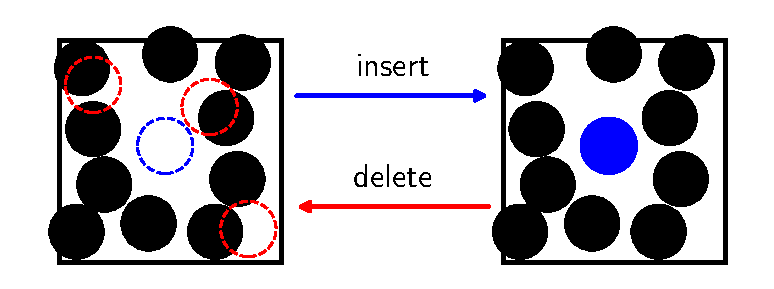
\includegraphics[width=6.5cm]{../figures/muvt_cb.pdf}
\caption{
Multiple first bead configurational bias insertion and deletion considers randomly-generated positions for a newly inserted particle, shown by the dashed circles, in an existing fluid of particles, shown by the black circles.
The most favorable position has the highest Rosenbluth probability of selection, which is shown in blue due to excluded volume overlap of the other red positions with the existing fluid.
The deletion step does not consider other positions or particles for deletion, but to obey detailed balance, the Rosenbluth factor in the deletion step includes the existing position as well as other randomly-generated positions.
}
\label{fig:muvt_cb}
\end{centering}
\end{figure}

The forward and reverse transition probabilities are summarized in Table~\ref{tab:lhs_ins_cb}.
Because the insertion is chosen as the forward transition, deletions are chosen among $N_i+1$ particles, where $N_i$ is the number of particles of type $i$ as defined from the old microstate.

\begin{table}
\begin{center}
\begin{tabular}{|c|c|}
 \hline
 \thead{Forward} & \thead{$\alpha_{o\rightarrow n}$} \\
 \hline
 Choose insert & $1/2$ \\
 \hline
 \makecell{Choose ${c}$ positions in $V$. \\ Probability that $\mathbf{r}_n$ is in ${c}$.} & ${c}\diff\mathbf{r}/V$ \\
 \hline
 Choose $\mathbf{r}_n$ from ${c}$ positions & $\pi_{cn}$ \\
 \hline
 Choose orientation & $P_{\omega n}\diff\boldsymbol{\omega}$ \\
 \hline\hline
 \thead{Reverse} & \thead{$\alpha_{n\rightarrow o}$} \\ [0.5ex]
 \hline
 Choose delete & $1/2$ \\
 \hline
 Choose particle of type $i$ & $1/(N_i + 1)$ \\
 \hline
\end{tabular}
\caption{Configurational bias particle insertion transition probabilities.}
\label{tab:lhs_ins_cb}
\end{center}
\end{table}

Using Table~\ref{tab:lhs_ins_cb} and substituting Eq.~\ref{eq:rhs_muvt} into Eq.~\ref{eq:detailed_balance}, the acceptance probability for CB particle insertion is
\begin{equation}
\chi = \frac{Vz_i}{P_{\omega n}{c}(N_i+1)\pi_{cn}}e^{-\beta\Delta U}.
\label{eq:cb_insdel}
\end{equation}

There is remarkable flexibility as to the choice of $\mathbf{r}_n$ from $c$ positions, which determines $\pi_{cn}$.
Ideally, $\pi_{cn}$ biases configurations where the energy of interaction of (the first interaction site of) a new particle at $\mathbf{r}_n$ with all the particles in the old microstate, $U_n$, is favorable.
A natural choice is to Boltzmann weight the selection of $c$ positions, $\pi_{cn} \propto e^{-\beta U_n}$.
Normalizing such a probability results in the Rosenbluth factor,
\begin{equation}
\pi_{cn} = \frac{e^{-\beta U_n}}{W_{c}},
\label{eq:rosenbluth}
\end{equation}
where
\begin{equation}
W_{c}=\sum_{i}^{c} e^{-\beta U_i}.
\label{eq:wc}
\end{equation}
Substitution of Eq.~\ref{eq:rosenbluth} into Eq.~\ref{eq:cb_insdel} yields
\begin{equation}
\chi = \frac{Vz_i W_{c}}{P_{\omega n}{c}(N_i+1)}e^{-\beta(\Delta U - U_n)}.
\label{eq:lhs_ins_cb}
\end{equation}
This form of $\pi_{cn}$ is also convenient because $\Delta U - U_n$ only contains interaction energies beyond the center of the first site (e.g., if there were multiple sites).
If there are no other orientational or multiple site interactions beyond the first bead, $\Delta U = U_n$.

The deletion step is nearly the inverse of Eq.~\ref{eq:lhs_ins_cb}, except for two details regarding the definition of $N_i$ and $\pi_{co}$.
Consider the deletion as the forward transition, where the particle is randomly chosen from $N_i$ in the old microstate.
The typical Rosenbluth factor, $W_{c}$, is calculated to satisfy detailed balance, but plays no role in the choice of the particle for deletion.
The trial with the deletion as the forward transition is described in Table~\ref{tab:lhs_del_cb}.

\begin{table}
\begin{center}
\begin{tabular}{|c|c|}
 \hline
 \thead{Forward} & \thead{$\alpha_{o\rightarrow n}$} \\ [0.5ex]
 \hline
 Choose delete & $1/2$ \\
 \hline
 Choose particle of type $i$ & $1/N_i$ \\
 \hline\hline
 \thead{Reverse} & \thead{$\alpha_{n\rightarrow o}$} \\ [0.5ex]
 \hline
 Choose insert & $1/2$ \\
 \hline
 \makecell{Choose ${c}$ positions in $V$. \\ Probability that $\mathbf{r}_o$ is in ${c}$.} & ${c}\diff\mathbf{r}/V$ \\
 \hline
 Choose $\mathbf{r}_o$ from ${c}$ positions & $\pi_{co}$ \\
 \hline
 Choose orientation & $P_{\omega o}\diff\boldsymbol{\omega}$ \\
 \hline
\end{tabular}
\caption{Configurational bias particle deletion transition probabilities.}
\label{tab:lhs_del_cb}
\end{center}
\end{table}

Thus, for deletions, the acceptance criteria using the typical Rosenbluth factor is given by,
\begin{equation}
\chi = \frac{c N_i P_{\omega o}}{Vz_i W_{c}}e^{-\beta(\Delta U + U_o)},
\label{eq:lhs_del_cb}
\end{equation}
where $\mathbf{r}_o$, the original position of the deleted particle, is among the ${c}-1$ other randomly generated positions in $\pi_{co}$, and $U_o$ is the interaction energy of the particle at $\mathbf{r}_o$ that the trial is attempting to delete.
If there are no other orientational or multiple site interactions beyond the first bead, $\Delta U = - U_o$.

In the ideal gas limit, $U\rightarrow 0$, $W_{c}\rightarrow{c}$, and Eqs.~\ref{eq:lhs_ins_cb} and \ref{eq:lhs_del_cb} are equivalent to Eqs.~\ref{eq:lhs_ins} and \ref{eq:lhs_del}.
Ideal gas simulations are helpful in quickly testing a CB implementation for verification.
Although ${c}$ in Eqs.~\ref{eq:lhs_ins_cb} and \ref{eq:lhs_del_cb} may be incorporated into the chemical potential, this may lead to confusion and is not recommended if multiple kinds of $\mu VT$ trials are attempted.

For single-site isotropic particles, such as those interacting via the Lennard-Jones potential, the orientational term (see Section~\ref{sec:lhs_rotation}) results in $P_{\omega n} = 1$ (or can be incorporated into the definition of $z_i$).
Hence, this trial is not particularly efficient compared to simply conducting $c$ traditional insertion or deletion trials sequentially.
However, this method becomes more efficient when the calculation of $P_{\omega n}$ for more complex molecules is comparable or more expensive than the calculation of $W_{c}$ (e.g., using partial regrowth or orientational bias, etc).
Another efficient approach is to use a reference potential that is less expensive than the full potential with longer-range interactions, where the reference potential still contains the most relevant terms for sampling (e.g., excluded volume in a dense fluid).
Such a method is named dual-cut CB \cite{vlugt_improving_1998} as described in the next section.

%%%%%%%%%%%%%%%%%%%%%%%%%
\subsection{\label{sec:lhs_insdel_dccb}Dual-cut configurational bias (DCCB)}
%%%%%%%%%%%%%%%%%%%%%%%%%

DCCB \cite{vlugt_improving_1998} is derived in a nearly identical fashion as CB presented in Section~\ref{sec:lhs_insdel_cb}.
The only difference is that $\pi_{cn}$ in Eq.~\ref{eq:rosenbluth} no longer uses the energy of the system, $U$, but rather, the energy of a reference system, $U_{r}$, that is, ideally, less computationally expensive to calculate.
This reference system could have a shorter cutoff distance, as per the namesake of this method.
Or, it could have a different potential or a different number of interaction sites.
For example, a simulation of SPC/E water could use a reference potential of hard spheres centered on the oxygen, which is not only short range but also reduces the number of interaction sites.
Because $\pi_{cn}$ contains the reference potential, $U_{rn}$, the insertion acceptance is given by
\begin{equation}
\chi = \frac{Vz_i W_{{c}r}}{P_{\omega nr}{c}(N_i+1)}e^{-\beta(\Delta U - U_{rn})},
\label{eq:lhs_ins_dccb}
\end{equation}
where
\begin{equation}
W_{{c}r}=\sum_{i}^{c} e^{-\beta U_{ri}}
\label{eq:wcr}
\end{equation}
and $U_{ri}$ is the reference potential contribution of the particle in microstate $i$.
Similar to Section~\ref{sec:lhs_insdel_cb}, the deletion acceptance is the inverse of the insertion, except that $N_i+1 \rightarrow N_i$, and $\mathbf{r}_o$ is one of the $c$ randomly generated positions for the calculation of $W_{{c}r}$.

The orientational term, $P_{\omega nr}$, may also utilize the reference potential, or not.
In either case, $U_{rn}$ in Eq.~\ref{eq:lhs_ins_dccb} is the sum of the (reference) interaction energies of each of the microstates chosen from both $P_{\omega nr}$ and $W_{cr}$ when the typical Rosenbluth terms are used in the probabilities of selection.

%%%%%%%%%%%%%%%%%%%%%%%%%
\subsection{\label{sec:lhs_insdel_cavity}Cavity bias}
%%%%%%%%%%%%%%%%%%%%%%%%%

Particle insertions may be biased to specific regions according to the location of cavities in a dense fluid \cite{mezei_cavity-biased_1980, mezei_grand-canonical_1987, snurr_prediction_1993, ikeda_generalization_2024}.
The practical limitation of this method is that it may become computationally expensive to identify the cavities.
In one approach, a number of test points are randomly placed in the volume for each trial \cite{mezei_cavity-biased_1980, mezei_grand-canonical_1987, snurr_prediction_1993}.
An ensemble average of the fraction of test points found within cavities, $P_c$, is then multiplied with the volume to approximate the combined volume of the cavities.
An alternative approach is to overlay the simulation domain with a discrete grid of points, as shown in Fig.~\ref{fig:cavity}.
To improve efficiency, this grid of points could be continuously updated for each trial.
In this case, the fraction of the grid that is within at least one of the cavities times the volume of the entire domain is the approximate volume of the cavities, assuming an equally spaced grid with enough resolution.
When a randomly chosen grid point within a cavity is chosen, the inserted particle may be placed at a random position selected uniformly within the voxel nearest that grid point.
In the case of an absorbent and adsorbent material, grid points that are always in the impenetrable regions of the absorbent material may be ignored \cite{snurr_prediction_1993}.
For particles with multiple sites, it may be convenient to consider just one of the sites for this cavity bias step (e.g., only the oxygen in a water molecule \cite{zhang_computational_2017}).
Voronoi tessellations may also be used to identify cavity volumes \cite{sastry_statistical_1997}.
In addition, cavity bias can also be implemented efficiently in lattice simulations \cite{barnes_structure_2009}.

\begin{figure}
\begin{centering}
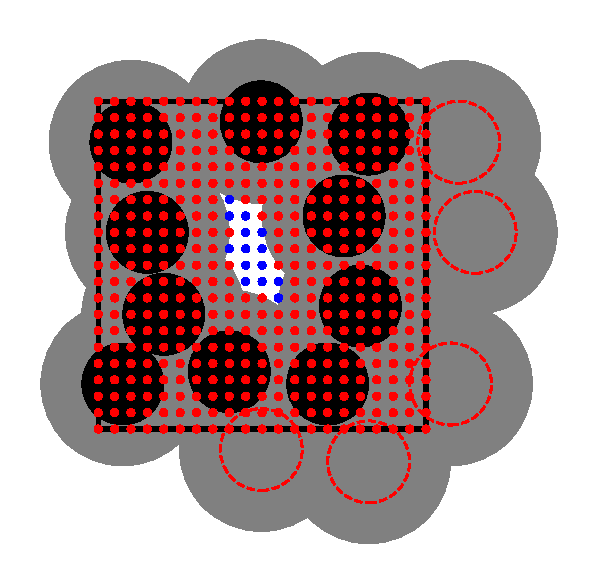
\includegraphics[width=6.5cm]{../figures/cavity.pdf}
\caption{
Cavity bias insertion and deletion may utilize a collection of points, here shown by a grid of red and blue points, which are tested for cavities.
Cavities are where another particle could fit without excluded volume overlap with existing particles, shown here as black circles with grey excluded volumes.
The red circles with dashed lines are periodic images, and the blue dots in the center are the only points in the grid that a new particle could be added onto without overlap.
}
\label{fig:cavity}
\end{centering}
\end{figure}

In this article, two variants of cavity bias will be derived.
In the first, a number of test points are chosen randomly in the domain to test for a cavity.
In the second, a predefined grid is used instead.

%%%%%%%%%%%%%%%%%%%%%%%%%
\subsubsection{\label{sec:lhs_insdel_cavity_random}Cavity bias with random test points}
%%%%%%%%%%%%%%%%%%%%%%%%%

A cavity bias trial with random test points proceeds as follows.
With equal probability, insertion or deletion of a particle of type $i$ is randomly chosen.
For insertion, $N_{test}$ points are chosen randomly in the simulation volume and $n_c$ of these points are determined to be within a cavity.
For hard particle systems, a cavity is well defined.
Soft particle systems require an ambiguous cavity definition that could affect sampling and efficiency (e.g., for the purposes of cavity determination, pick an arbitrary hard particle size for the soft particles).
Here, $n_c$ is computed for each set of randomly generated test points; the possibility of using an ensemble average of $n_c$ is discussed at the end of this section.
A particle of type $i$ is placed on one of the $n_c$ points.
For deletion, randomly choose a particle of type $i$ for removal.

With insertion as the forward transition, the transition probabilities are summarized in Table~\ref{tab:lhs_ins_cavity_random}.
Because the insertion is the forward transition, deletions are chosen among the $N_i+1$ particles, where $N_i$ is the number as defined from the old microstate.

\begin{table}
\begin{center}
\begin{tabular}{|c|c|}
 \hline
 \thead{Forward} & \thead{$\alpha_{o\rightarrow n}$} \\ [0.5ex]
 \hline
 Choose insert & $1/2$ \\
 \hline
 \makecell{Choose $N_{test}$ points in $V$.\\Probability $\mathbf{r}_n$ is in $N_{test}$.} & $N_{test}\diff\mathbf{r}/V$ \\
 \hline
 Choose $\mathbf{r}_n$ from $n_c$ & $1/n_c$ \\
 \hline
 Choose orientation & $P_{\omega n}\diff\boldsymbol{\omega}$ \\
 \hline\hline
 \thead{Reverse} & \thead{$\alpha_{n\rightarrow o}$} \\ [0.5ex]
 \hline
 Choose delete & $1/2$ \\
 \hline
 Choose particle of type $i$ & $1/(N_i+1)$ \\
 \hline
\end{tabular}
\caption{Cavity bias particle insertion transition probabilities with random test points.}
\label{tab:lhs_ins_cavity_random}
\end{center}
\end{table}

Using Table~\ref{tab:lhs_ins_cavity_random} and substituting Eq.~\ref{eq:rhs_muvt} into Eq.~\ref{eq:detailed_balance}, the acceptance probability for cavity bias particle insertion is
\begin{equation}
\chi = \left(\frac{n_c}{N_{test}}\right) \frac{z_i V}{P_{\omega n}(N_i+1)}e^{-\beta\Delta U}.
%\label{eq:dccb_insdel}
\end{equation}
For comparison to previously published articles, the probability that a random test point is in the cavity is given by $P_c = n_c/N_{test}$ \cite{mezei_cavity-biased_1980, mezei_grand-canonical_1987, snurr_prediction_1993}.
With deletion as the forward transition, the transition probabilities are summarized in Table~\ref{tab:lhs_del_cavity_random}.

\begin{table}
\begin{center}
\begin{tabular}{|c|c|}
 \hline
 \thead{Forward} & \thead{$\alpha_{o\rightarrow n}$} \\ [0.5ex]
 \hline
 Choose delete & $1/2$ \\
 \hline
 Choose particle of type $i$ & $1/N_i$ \\
 \hline\hline
 \thead{Reverse} & \thead{$\alpha_{n\rightarrow o}$} \\ [0.5ex]
 \hline
 Choose insert & $1/2$ \\
 \hline
 \makecell{Choose $N_{test}$ points in $V$.\\Probability $\mathbf{r}_o$ is in $N_{test}$.} & $N_{test}\diff\mathbf{r}/V$ \\
 \hline
 Choose $\mathbf{r}_o$ from $n_c$ & $1/n_c$ \\
 \hline
 Choose orientation & $P_{\omega o}\diff\boldsymbol{\omega}$ \\
 \hline
\end{tabular}
\caption{Cavity bias particle deletion transition probabilities with random test points.}
\label{tab:lhs_del_cavity_random}
\end{center}
\end{table}

Using Table~\ref{tab:lhs_del_cavity_random} and substituting Eq.~\ref{eq:rhs_muvt} into Eq.~\ref{eq:detailed_balance}, the acceptance probability for cavity bias particle deletions is
\begin{equation}
\chi = \frac{N_{test}}{n_c}\left(\frac{N_i P_{\omega o}}{z_i V}\right)e^{-\beta\Delta U},
\label{eq:energy_bias_del}
\end{equation}
where $n_c$ must be computed after the particle is deleted and the $N_{test}$ points includes the original position of the particle, $\mathbf{r}_o$.
For hard particle systems, a cavity is well defined and $n_c$ in the deletion step would never be zero because it includes $\mathbf{r}_o$.
But for soft interactions, depending on the definition of the cavity, $n_c$ may be zero.
If $n_c$ is zero, the trial should be rejected or else detailed balance is violated because the reverse transition is impossible.

For comparison to previously published articles \cite{mezei_cavity-biased_1980, mezei_grand-canonical_1987, snurr_prediction_1993}, it is not clear if $\mathbf{r}_o$ was included in one of the $N_{test}$ points during the deletion step.
The previous work also computed an ensemble average of $n_c$ over many trials rather than computing an instantaneous $n_c$.
An ensemble average of $n_c$ has the benefit of possibly requiring fewer $N_{test}$ points.
On the other hand, it is beyond the scope of this article to prove whether or not an ensemble average $n_c$ introduces biases via violation of detailed balance~\cite{ikeda_generalization_2024}.
The previous work also interpolated the cavity probability from other state points in special cases, and introduced unbiased insertion and deletion trials when $n_c=0$.

%%%%%%%%%%%%%%%%%%%%%%%%%
\subsubsection{\label{sec:lhs_insdel_cavity_testpoint}Cavity bias with a predefined list}
%%%%%%%%%%%%%%%%%%%%%%%%%

While Section~\ref{sec:lhs_insdel_cavity_random} used random points, a predefined list or grid, as shown in Fig.~\ref{fig:cavity}, is considered in this section.
The benefit of using a predefined list is that certain points could be removed if, for example, those grid points could never be in a cavity because of the location of a rigid wall or obstacle (e.g., an adsorbent material).
A grid is created with spacing $\delta$ in each dimension, and after points not amenable to insertion are removed, there are $N_l$ points remaining in the predefined list.

A cavity bias trial with a predefined list proceeds as follows.
With equal probability, insertion or deletion of a particle of type $i$ is randomly chosen.
For an insertion, $N_{test}$ points are randomly chosen from the fixed list of $N_l$ points, and $n_c$ of those $N_{test}$ points are determined to be within a cavity.
One of these $n_c$ points is randomly chosen, denoted as $\mathbf{r}_{nl}$.
The inserted particle of type $i$ is then placed at a random position selected uniformly within $\pm 0.5\delta$ of $\mathbf{r}_{nl}$ in each dimension.
For a deletion, randomly choose a particle of type $i$ and remove it.
In order to obey detailed balance, deletion attempts of particles that are not within $\pm 0.5\delta$ of a point in $N_l$ must be immediately rejected (e.g., if some grid points were removed yet fluid particles managed to exist in the vicinity of those removed points).
Otherwise, particles could be removed from the system where insertions could not immediately place them back for the reverse trial.

With insertion as the forward transition, the transition probabilities are summarized in Table~\ref{tab:lhs_ins_cavity_testpoint}.
Because the insertion is the forward transition, deletions are chosen among the $N_i+1$ particles, where $N_i$ is the number of particles of type $i$ as defined from the old microstate.

\begin{table}
\begin{center}
\begin{tabular}{|c|c|}
 \hline
 \thead{Forward} & \thead{$\alpha_{o\rightarrow n}$} \\ [0.5ex]
 \hline
 Choose insert & $1/2$ \\
 \hline
 \makecell{Choose $N_{test}$ points from $N_l$.\\Probability $\mathbf{r}_{nl}$ is in $N_{test}$} & $N_{test}/N_l$ \\
 \hline
 Choose $\mathbf{r}_{nl}$ from $n_c$ & $1/n_c$ \\
 \hline
 Choose $\mathbf{r}_n$ about $\mathbf{r}_{nl}$ & $\diff\mathbf{r}/\delta^D$ \\
 \hline
 Choose orientation & $P_{\omega n}\diff\boldsymbol{\omega}$ \\
 \hline\hline
 \thead{Reverse} & \thead{$\alpha_{n\rightarrow o}$} \\ [0.5ex]
 \hline
 Choose delete & $1/2$ \\
 \hline
 Choose particle of type $i$ & $1/(N_i+1)$ \\
 \hline
\end{tabular}
\caption{Cavity bias particle insertion transition probabilities with a predefined list.}
\label{tab:lhs_ins_cavity_testpoint}
\end{center}
\end{table}

Using Table~\ref{tab:lhs_ins_cavity_testpoint} and substituting Eq.~\ref{eq:rhs_muvt} into Eq.~\ref{eq:detailed_balance}, the acceptance probability for cavity bias particle insertion with $N_{test}$ points is
\begin{equation}
\chi = N_l \delta^D\left(\frac{n_c}{N_{test}}\right)\frac{z_i}{P_{\omega n}(N_i+1)}e^{-\beta\Delta U}.
\label{eq:cavity_bias_ntest}
\end{equation}
This equation takes the form of Eq.~4 of Ref.~\cite{snurr_prediction_1993} because the fraction of the points in the cavity is $P_c = n_c/N_{test}$ and the total volume considered for insertions is $v=N_l\delta^D$.

With deletion as the forward transition, the position of the chosen particle to be deleted is $\mathbf{r}_o$, which is within $\delta$ in each dimension of a point within the predefined list, $\mathbf{r}_{ol}$.
If not, the deletion is rejected to obey detailed balance.
The transition probabilities are summarized in Table~\ref{tab:lhs_del_cavity_testpoint}.

\begin{table}
\begin{center}
\begin{tabular}{|c|c|}
 \hline
 \thead{Forward} & \thead{$\alpha_{o\rightarrow n}$} \\ [0.5ex]
 \hline
 Choose delete & $1/2$ \\
 \hline
 Choose particle of type $i$ & $1/N_i$ \\
 \hline\hline
 \thead{Reverse} & \thead{$\alpha_{n\rightarrow o}$} \\ [0.5ex]
 \hline
 Choose insert & $1/2$ \\
 \hline
 \makecell{Choose $N_{test}$ from $N_l$ points.\\Probability $\mathbf{r}_{ol}$ is in $N_{test}$} & $N_{test}/N_l$ \\
 \hline
 Choose $\mathbf{r}_{ol}$ from $n_c$ & $1/n_c$ \\
 \hline
 Choose $\mathbf{r}_o$ about $\mathbf{r}_{ol}$ & $\diff\mathbf{r}/\delta^D$ \\
 \hline
 Choose orientation & $P_{\omega o}\diff\boldsymbol{\omega}$ \\
 \hline
\end{tabular}
\caption{Cavity bias particle deletion transition probabilities with a predefined list.}
\label{tab:lhs_del_cavity_testpoint}
\end{center}
\end{table}

Using Table~\ref{tab:lhs_del_cavity_testpoint} and substituting Eq.~\ref{eq:rhs_muvt} into Eq.~\ref{eq:detailed_balance}, the acceptance probability for cavity bias particle deletions with $N_{test}$ points is
\begin{equation}
\chi = \frac{1}{N_l \delta^D}\left(\frac{N_{test}}{n_c}\right)\frac{N_i P_{\omega o}}{z_i}e^{-\beta\Delta U}.
\label{eq:cavity_bias_ntest_del}
\end{equation}
Similar to Eq.~\ref{eq:energy_bias_del}, $n_c$ is computed after the particle is deleted and includes $\mathbf{r}_{ol}$, which is the closest grid point to the old macrostate position of the deleted particle, $\mathbf{r}_o$.

%%%%%%%%%%%%%%%%%%%%%%%%%
\subsection{\label{sec:lhs_insdel_energybias}Energy bias}
%%%%%%%%%%%%%%%%%%%%%%%%%

Particle insertions may also be biased in specific regions according to their energy of interaction with a fixed adsorbent material \cite{snurr_prediction_1993}, as illustrated in Fig.~\ref{fig:energybias}.
The simulation volume is divided into a number of small voxels with volume $v$.
Energy bias particle insertions and deletions proceed as follows.
With equal probability, an insertion or deletion is attempted.
For an insertion, a voxel is randomly chosen with probability $P_c$.
A new particle of type $i$ is then randomly placed inside of the chosen voxel.
For a deletion, an existing particle of type $i$ is chosen randomly and removed from the system.
The trial probabilities are summarized with insertion as the forward transition in Table~\ref{tab:lhs_ins_energybias}.

\begin{figure}
\begin{centering}
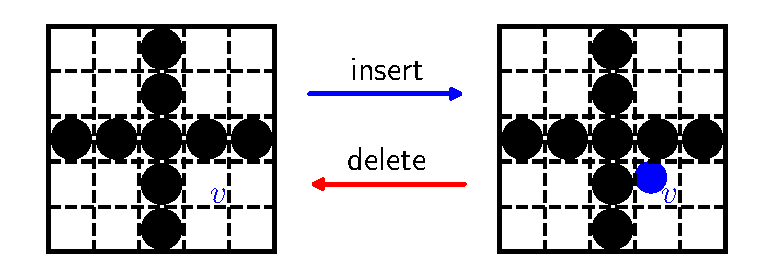
\includegraphics[width=6.5cm]{../figures/energybias.pdf}
\caption{
Energy bias insertion and deletion \cite{snurr_prediction_1993} divides the simulation domain into voxels, with $25$ shown here by the dashed lines.
One voxel, $v$, is chosen for the available insertion volume according to a probability Boltzmann-weighted by the energy of interaction with a rigid adsorbent frame, shown by the black circles.
The reverse move is when the newly inserted fluid particle, shown in blue, is randomly chosen for deletion among all the fluid particles.
}
\label{fig:energybias}
\end{centering}
\end{figure}

\begin{table}
\begin{center}
\begin{tabular}{|c|c|}
 \hline
 \thead{Forward} & \thead{$\alpha_{o\rightarrow n}$} \\ [0.5ex]
 \hline
 Choose insert & $1/2$ \\
 \hline
 Choose voxel & $P_c$ \\
 \hline
 Choose position in $v$ & $\diff\mathbf{r}/v$ \\
 \hline
 Choose orientation & $P_{\omega n}\diff\boldsymbol{\omega}$ \\
 \hline\hline
 \thead{Reverse} & \thead{$\alpha_{n\rightarrow o}$} \\ [0.5ex]
 \hline
 Choose delete & $1/2$ \\
 \hline
 Choose particle of type $i$ & $1/(N_i+1)$ \\
 \hline
\end{tabular}
\caption{Energy bias particle insertion transition probabilities.}
\label{tab:lhs_ins_energybias}
\end{center}
\end{table}

Substituting Eq.~\ref{eq:rhs_muvt} into the first ratio in Eq.~\ref{eq:detailed_balance}, and using Table~\ref{tab:lhs_ins_energybias} for the second ratio in Eq.~\ref{eq:detailed_balance}, results in
\begin{equation}
\chi = \frac{v z_i}{P_{\omega n}(N_i+1)P_c} e^{-\beta\Delta U}
\label{eq:lhs_ins_energybias}
\end{equation}
for energy bias insertions.
Deletions as the forward trial is summarized in Table~\ref{tab:lhs_del_energybias}.

\begin{table}
\begin{center}
\begin{tabular}{|c|c|}
 \hline
 \thead{Forward} & \thead{$\alpha_{o\rightarrow n}$} \\ [0.5ex]
 \hline
 Choose delete & $1/2$ \\
 \hline
 Choose particle of type $i$ & $1/N_i$ \\
 \hline\hline
 \thead{Reverse} & \thead{$\alpha_{n\rightarrow o}$} \\ [0.5ex]
 \hline
 Choose insert & $1/2$ \\
 \hline
 Choose voxel & $P_c$ \\
 \hline
 Choose position in $v$ & $\diff\mathbf{r}/v$ \\
 \hline
 Choose orientation & $P_{\omega o}\diff\boldsymbol{\omega}$ \\
 \hline
\end{tabular}
\caption{Energy bias particle deletion transition probabilities.}
\label{tab:lhs_del_energybias}
\end{center}
\end{table}

Substituting Eq.~\ref{eq:rhs_muvt} into the first ratio in Eq.~\ref{eq:detailed_balance}, and using Table~\ref{tab:lhs_del_energybias} for the second ratio in Eq.~\ref{eq:detailed_balance}, results in
\begin{equation}
\chi = \frac{N_i P_c P_{\omega o}}{v z_i} e^{-\beta\Delta U}
\label{eq:lhs_del_energybias}
\end{equation}
for deletions as the reverse of energy bias insertions.

For both insertions and deletions, a suitable $P_c$ must be utilized that is ideally inexpensive to compute and increases sampling in the desired location.
As originally formulated, a good choice for $P_c$ is to weight the probability by the Boltzmann factor of the energy a particle in the center of the chosen target volume, $v$, would have with an adsorbent material, $U^a_t$,
\begin{equation}
P_c = \frac{e^{-\beta U^a_t}}{\sum_i e^{-\beta U^a_i}}.
\label{eq:lhs_energybias_pt}
\end{equation}

%%%%%%%%%%%%%%%%%%%%%%%%%
\subsection{\label{sec:lhs_insdel_subset}Insertion and deletion in a targeted region}
%%%%%%%%%%%%%%%%%%%%%%%%%

Particle insertions and deletions may also be performed in a targeted region, $v$, shown in Fig.~\ref{fig:muvt_target} with a rigid adsorbent framework.
The trial proceeds as follows.
First, a particle insertion or deletion trial is chosen randomly with equal probability.
If a particle insertion trial is chosen, then a particle of type $i$ is placed at a random position selected uniformly in a targeted region, $v$, with random orientation.
If a particle deletion trial is chosen, then a random particle of type $i$ within $v$ is chosen for removal.
Here, $n_i$ is the number of particles of type $i$ inside $v$ at the beginning of the trial.
For particle deletions, if $n_i=0$, then reject the trial.
To obey detailed balance, $v$ cannot change during the trial.
The transition probability of an insertion trial as the forward transition is then summarized in Table~\ref{tab:lhs_ins_subset}.

\begin{figure}
\begin{centering}
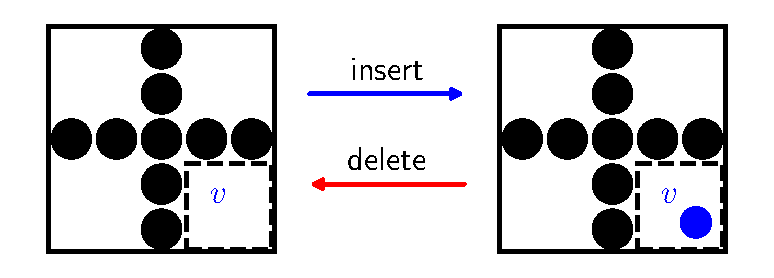
\includegraphics[width=6.5cm]{../figures/muvt_target.pdf}
\caption{
Insertion and deletion trials in a targeted region, $v$.
Similar to Fig.~\ref{fig:energybias}, the targeted region could be carefully chosen to avoid excluded volume overlap with a rigid adsorbent framework.
}
\label{fig:muvt_target}
\end{centering}
\end{figure}

\begin{table}
\begin{center}
\begin{tabular}{|c|c|}
 \hline
 \thead{Forward} & \thead{$\alpha_{o\rightarrow n}$} \\ [0.5ex]
 \hline
 Choose insert & $1/2$ \\
 \hline
 Choose position in $v$ & $\diff\mathbf{r}/v$ \\
 \hline
 Choose orientation & $P_{\omega n}\diff\boldsymbol{\omega}$ \\
 \hline\hline
 \thead{Reverse} & \thead{$\alpha_{n\rightarrow o}$} \\ [0.5ex]
 \hline
 Choose delete & $1/2$ \\
 \hline
 Choose particle of type $i$ in $v$ & $1/(n_i+1)$ \\
 \hline
\end{tabular}
\caption{Particle insertion transition probabilities in a targeted region.}
\label{tab:lhs_ins_subset}
\end{center}
\end{table}

Substituting Eq.~\ref{eq:rhs_muvt} into the first ratio in Eq.~\ref{eq:detailed_balance}, and using Table~\ref{tab:lhs_ins_subset} for the second ratio in Eq.~\ref{eq:detailed_balance}, results in
\begin{equation}
\chi = \frac{v z_i}{P_{\omega n}(n_i+1)} e^{-\beta\Delta U},
\label{eq:lhs_ins_target}
\end{equation}
where $n_i$ is defined as the number of particles of type $i$ inside $v$ at the beginning of the insertion trial (i.e., before insertion).
The transition probability of a deletion trial as the forward transition is then summarized in Table~\ref{tab:lhs_del_subset}.

\begin{table}
\begin{center}
\begin{tabular}{|c|c|}
 \hline
 \thead{Forward} & \thead{$\alpha_{o\rightarrow n}$} \\ [0.5ex]
 \hline
 Choose delete & $1/2$ \\
 \hline
 Choose particle of type $i$ in $v$ & $1/n_i$ \\
 \hline\hline
 \thead{Reverse} & \thead{$\alpha_{n\rightarrow o}$} \\ [0.5ex]
 \hline
 Choose insert & $1/2$ \\
 \hline
 Choose position in $v$ & $\diff\mathbf{r}/v$ \\
 \hline
 Choose orientation & $P_{\omega o}\diff\boldsymbol{\omega}$ \\
 \hline
\end{tabular}
\caption{Particle deletion transition probabilities in a targeted region.}
\label{tab:lhs_del_subset}
\end{center}
\end{table}

Substituting Eq.~\ref{eq:rhs_muvt} into the first ratio in Eq.~\ref{eq:detailed_balance}, and using Table~\ref{tab:lhs_del_subset} for the second ratio in Eq.~\ref{eq:detailed_balance}, results in
\begin{equation}
\chi = \frac{n_i P_{\omega o}}{v z_i} e^{-\beta\Delta U},
\label{eq:lhs_del_target}
\end{equation}
where $n_i$ is defined as the number of particles of type $i$ inside $v$ at the beginning of the deletion trial (i.e., before deletion).

%%%%%%%%%%%%%%%%%%%%%%%%%
\subsection{\label{sec:lhs_insdel_avb}Aggregation volume bias (AVB)}
%%%%%%%%%%%%%%%%%%%%%%%%%

\begin{figure}
\begin{centering}
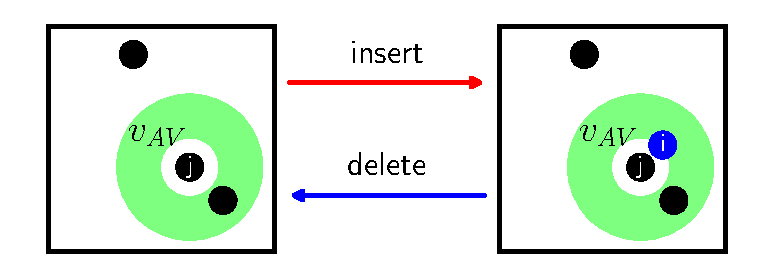
\includegraphics[width=6.5cm]{../figures/avb.pdf}
\caption{
Insertion and deletion of a blue particle of type $i$ within the aggregation volume (AV), shown in green, of an existing particle of type $j$.
}
\label{fig:avb_gce}
\end{centering}
\end{figure}

AVB insertions and deletions specifically target the positions near other molecules \cite{chen_improving_2001} in order to improve sampling for aggregated clusters of molecules, as shown in Fig.~\ref{fig:avb_gce}.
In these derivations, aggregation volumes (AVs) are defined uniquely by one specific interaction site on a target particle and one specific site on a mobile particle.
A single site should be specifically defined, not a type of site when there are multiple sites of the same type, or else detailed balance may be broken.
Instead, if multiple AVs are desired in a single target particle, then simply treat each as a separate trial.
For an isotropic AV, the mobile particle is inside the AV of the target particle if the distance between the two sites is between $r_{inner}$ and $r_{outer}$.

An attempted AVB insertion and deletion proceeds as follows.
First, an insertion or deletion trial is chosen randomly with equal probability.
If a particle insertion is chosen, then the new position, $\mathbf{r}_n$, of an interaction site of the new particle of type $i$ is placed at a random position selected uniformly within the AV, $v_{AV}$, of a different particle of type $j$ that is randomly chosen from among $N_j$ particles.
The AV, in this example, is defined using the spherical shell between $r_{inner}$ and $r_{outer}$, although it is possible to define an orientation-specific AV \cite{rovigatti_how_2018}.
See Section~\ref{sec:spherical_shell} for how to generate randomly uniform points in a spherical shell.
The remaining sites in the new particle may be oriented randomly about $\mathbf{r}_n$ or regrown with CB.
If a particle deletion is chosen, then a particle of type $j$ is randomly chosen.
A random particle of type $i$ within the AV of the chosen particle of type $j$ is removed from among the $N_i^{AV}$ particles of type $i$ within the AV.
The transition probabilities with insertion as the forward transition is summarized in Table~\ref{tab:lhs_ins_avb}.

\begin{table}
\begin{center}
\begin{tabular}{|c|c|}
 \hline
 \thead{Forward} & \thead{$\alpha_{o\rightarrow n}$} \\ [0.5ex]
 \hline
 Choose insert & $1/2$ \\
 \hline
 Choose particle of type $j$ & $1/N_j$ \\
 \hline
 Choose $\mathbf{r}_n$ in AV & $\diff\mathbf{r}/v_{AV}$ \\
 \hline
 Choose orientation & $P_{\omega n}\diff\boldsymbol{\omega}$ \\
 \hline\hline
 \thead{Reverse} & \thead{$\alpha_{n\rightarrow o}$} \\ [0.5ex]
 \hline
 Choose delete & $1/2$ \\
 \hline
 Choose particle of type $j$ & $1/(N_j + \delta_{ij})$ \\
 \hline
 Choose interaction site in AV& $1/(N_i^{AV} + 1)$ \\
 \hline
\end{tabular}
\caption{AVB particle insertion transition probabilities.}
\label{tab:lhs_ins_avb}
\end{center}
\end{table}

If particle type $i$ and $j$ are identical, then $\delta_{ij}=1$.
Otherwise, $\delta_{ij}=0$.
Substituting Eq.~\ref{eq:rhs_muvt} into the first ratio in Eq.~\ref{eq:detailed_balance}, and using Table~\ref{tab:lhs_ins_avb} for the second ratio in Eq.~\ref{eq:detailed_balance}, results in
\begin{equation}
\chi = \frac{N_j}{N_j+\delta_{ij}}\left[\frac{v_{AV}z_i}{P_{\omega n}(N_i^{AV}+1)}\right] e^{-\beta\Delta U}.
\label{eq:lhs_gc_avb_add}
\end{equation}

Deletions are derived in an identical fashion, except that $N^{AV}_i$ is evaluated from the perspective of the state before the deletion (e.g., after insertions), and the trial is summarized in Table~\ref{tab:lhs_del_avb}.
The deletion acceptance is obtained by substituting Eq.~\ref{eq:rhs_muvt} into the first ratio in Eq.~\ref{eq:detailed_balance}, and using Table~\ref{tab:lhs_del_avb} for the second ratio in Eq.~\ref{eq:detailed_balance}, resulting in
\begin{equation}
\chi = \frac{N_j}{N_j-\delta_{ij}}\left(\frac{N^{AV}_i P_{\omega o}}{v_{AV}z_i}\right)e^{-\beta\Delta U}.
\label{eq:lhs_gc_avb_del}
\end{equation}

\begin{table}
\begin{center}
\begin{tabular}{|c|c|}
 \hline
 \thead{Forward} & \thead{$\alpha_{o\rightarrow n}$} \\ [0.5ex]
 \hline
 Choose delete & $1/2$ \\
 \hline
 Choose particle of type $j$ & $1/N_j$ \\
 \hline
 Choose interaction site in AV& $1/N_i^{AV}$ \\
 \hline\hline
 \thead{Reverse} & \thead{$\alpha_{n\rightarrow o}$} \\ [0.5ex]
 \hline
 Choose insert & $1/2$ \\
 \hline
 Choose particle of type $j$ & $1/(N_j - \delta_{ij})$ \\
 \hline
 Choose $\mathbf{r}_o$ in AV & $\diff\mathbf{r}/v_{AV}$ \\
 \hline
 Choose orientation & $P_{\omega o}\diff\boldsymbol{\omega}$ \\
 \hline
\end{tabular}
\caption{AVB particle deletion transition probabilities.}
\label{tab:lhs_del_avb}
\end{center}
\end{table}
